	\chapter{Regression and Classification}
	\section{Linear Regression}
Residuals are the distance from the data point to the fitted line or linear regression.

Mean square of errors
	\begin{equation}
		m_e = \frac{\sum \left(y_i - y_p\right)^2}{n-2} = \frac{\sum e_i^2}{n-2}
	\end{equation}

Standard deviation of the residuals, also called the root mean square of the errors.

	\begin{equation}
		s_e = \sqrt{\frac{\sum \left(y_i - y_p\right)^2}{n-2}} = \sqrt{\frac{\sum e_i^2}{n-2}} = \sqrt{m_e}
	\end{equation}

Mean absolute error
	\begin{equation}
		a_e = \frac{\sum \left|y_i - y_p\right|}{n-2} = \frac{\sum \left|e_i\right|}{n-2}
	\end{equation}

	\begin{mathwhere}
		\mathdefitem{y_i}{actual value;}
		\mathdefitem{y_p}{predicted value;}
		\mathdefitem{e}{residual;}
		\mathdefitem{n}{number of observations/samples.}
	\end{mathwhere}

Coefficient of determination, often call the R squared score, is the proportion of the variation in the dependent variable that is predictable from the independent variable(s).  A score of 1 means the variance is perfectly captured.

As more parameters are added to the model, the R squared score will increase.  Even if the parameters does not correlate well with the output, by chance it can improve the result.

Adjusted R squared is a modification to R squared to create a more intuitive response to adding model parameters.  If the added parameter improves the response, the adjusted R square value goes up.  If it does not add \emph{enough} value to the response, the adjusted R square value falls.

	\subsection{Over Fit and Under Fit}
An over fit model will capture noise as well as the information.  An under fit model will not capture the available information.

	\subsubsection{R Square Score}
If the model is over fit, the R squared score on the training data and the testing data will not match well.


	\section{Logistic Regression}
Logistic regression is a classification problem.

	\subsection{Understanding TP, TN, FP, and FN}
The second entry is the models prediction.  The first entry is whether that prediction is correct.
	\begin{equation}
		(T/F)(P/N) = (\textrm{was the prediction correct})(\textrm{model prediction})
	\end{equation}

A FP is also called a Type 1 Error.  A FN is also called a Type 2 Error.

	\subsection{Section FAQ}

	\resetquestioncounter{}
    \begin{qanda}
\question{When should we use Precision or Recall as model performance evaluation criteria?}

\answer{Precision should be used when you want to minimize False Positives i.e. one wants at least negatives should not be predicted as positives. Also, in cases where the loss of resources is high.  Recall should be used when you want to minimize False Negatives, i.e. one wants at least positives should not be predicted as negatives. Also, in cases where the loss of opportunity is high.}
    \end{qanda}

    \begin{qanda}
		\question{What is misclassification?}

		\answer{Misclassification occurs when values are predicted incorrectly or the model assigns the observation to a different class instead of the class it should be in. For example, for observation, the actual label is class 0 but the model predicts this observation as class 1.}
    \end{qanda}

    \begin{qanda}
		\question{Why confusion matrix is inverted in the hands-on notebook and it is difficult to identify TP, TN, FP, and FN?}
		\answer{Generally, in theory, or while teaching confusion matrix many sources keep the predicted labels are on the y-axis whereas the actual labels are on the x-axis. But in the implementation, it can be different depending upon the library we are using.  Sklearn follows an approach of Actual labels on the x-axis and Predicted labels on the y-axis.  Let us understand how to identify TP, TN, FP, and FN in a confusion matrix through an example.  Let's say we are trying to predict a person is diabetic (class 1) or not (class 0).
	\begin{bulletedlist}
		\item True Positives (TP): A person has diabetes and the model predicted that person is diabetic.
		\item True Negatives (TN): A person doesn't have diabetes and the model predicted that person doesn't have diabetes.
		\item False Positives (FP): A person doesn't have diabetes but the model predicted that person has diabetes.
		\item False Negatives (FN): The person has diabetes but the model predicted that person doesn't have diabetes.
	\end{bulletedlist}
Now based on the actual label and predicted label you can identify the TP, TN, FP, and FN.}
    \end{qanda}




    \begin{qanda}
		\question{When do we label encode and create dummy variables for categorical levels?}

		\answer{We generally prefer label encoding when there is a sense of order on the values, for example, let's say a variable has values bad, good, very good in such a case we know that there is an order and we can encode them as 1, 2, and 3 respectively.  But let's say the values are red, blue, green in this case there is no definite order in values and hence creating dummy variables would be a better choice.}
    \end{qanda}

Use Sigmoid functions because of the S-shape.

Advantages
	\begin{bulletedlist}
		\item A classification model that gives probabilities.
		\item Easily extended to multiple classes (multinomial regression).
		\item Quick to train and very fast at classifying unknown records.
	\end{bulletedlist}


Disadvantages
	\begin{bulletedlist}
		\item Construction linear boundaries.
		\item Assumes that variables are independent (does not include interaction terms).
		\item Interpretation of coefficients is difficult.
	\end{bulletedlist}


    \subsection{Logit Regression}
    \begin{bulletedlist}
		\item This is the most popular model.
		\item It must be between 0 and 1.
    \end{bulletedlist}

	\begin{equation}
		y = \frac{1}{1+e^{-\left(a+bx\right)}} = \frac{e^{\left(a+bx\right)}}{1+e^{\left(a+bx\right)}}
	\end{equation}
Or equivalently
	\begin{equation}
		\log\left(\frac{y}{1-y}\right) = a+bx
	\end{equation}
which can be interpreted as the log of the probability odds is a linear function.

Solving for a and b is not done by minimizing the errors.  Because the function is a non-linear function, multiple curves can be produced (called a non-convex problem?).  Instead, the solution is found by minimizing the log loss (cross entropy) which is defined as
	\begin{equation}
		-y\log\left(\hat{y}\right) - \left(1-y\right)\log\left(1-\hat{y}\right)
	\end{equation}
	\begin{mathwhere}[0.49in]
		\mathdefitem{y}{observed objective value;}
		\mathdefitem{\hat{y}}{predicted objective value.}
	\end{mathwhere}


	\subsection{Probit Regression}
	\begin{equation}
		y = \Phi\left(x\right)
	\end{equation}
	\begin{mathwhere}[0.49in]
		\mathdefitem{\Phi\left(x\right)}{cumulative function of the normal distribution.}
	\end{mathwhere}


	\subsection{Evaluation of Models}
Recall, sensitivity, and true positive rate are the same thing.  Specificity and true negative rate are the same thing.  Maximizing sensitivity and specificity at the same time means minimizing the false negatives and false positives.
	\begin{eqnarray}
		\textrm{accuracy} 						& = & 1 - \textrm{error} 						\\
												& = & \frac{T_P + T_N}{T_P + T_N + F_N + F_P} 	\\
		\textrm{classification error  rate}		& = & 1 - \textrm{accuracy} 					\\
												& = & \frac{F_P + F_N}{T_P + T_N + F_N + F_P} 	\\
		\textrm{recall/sensitivity}				& = & \frac{T_P}{T_P + F_N} 					\\
		\textrm{precision} 						& = & \frac{T_P}{T_P + F_P} 					\\
		\textrm{specificity} 					& = & \frac{T_N}{T_N + F_P}						\\
		\falsepositiverate						& = & \frac{F_P}{T_N + F_P}						\\
												& = & 1 - \textrm{specificity}					\\
		\textrm{gini}							& = & \frac{A_c - 0.5}{0.5}						\\
												& = & 2A_c - 1									\\
		F1										& = & \frac{2*\textrm{precision} * \textrm{recall}}
                                                             {\textrm{precision} + \textrm{recall}}
	\end{eqnarray}
	\begin{mathwhere}[0.4in]
		\mathdefitem{T_N}{true negatives;}
		\mathdefitem{T_P}{true positives;}
		\mathdefitem{F_N}{false negatives;}
		\mathdefitem{F_P}{false positives;}
		\mathdefitem{A_c}{area under the curve.}
	\end{mathwhere}

Accuracy is the percent of the positive and negatives accurately predicted out of the totals.  When dealing with imbalanced data, this can be misleading because the class with the smaller number of entries can be ignored and the accuracy can still be good.  For example, if you are trying to predict if a loan will be defaulted on and 98 percent of people do not default, they just predict everyone does not default and you can get a good accuracy score.

Recall (sensitivity/true positive rate): Percent of the positives that were caught.  For example, what percent of people who have a disease did a medical test catch.

Specificity: Percent of the negatives that were caught (correctly labeled).

Precision talks about how precise/accurate your model is out of those \emph{predicted positive}, how many of them are \emph{actual positive}.
Precision is a good measure to determine, when the costs of \emph{false positive} is high. For instance, email spam detection. In email spam detection, a false positive means that an email that is non-spam (\emph{actual negative}) has been identified as spam (predicted spam). The email user might lose important emails if the precision is not high for the spam detection model.

Recall actually calculates how many of the \emph{actual positives} our model capture through labeling it as positive (\emph{true positive}). Applying the same understanding, we know that recall shall be the model metric we use to select our best model when there is a high cost associated with \emph{false negative}.  For instance, in fraud detection or sick patient detection. If a fraudulent transaction (\emph{actual positive}) is predicted as non-fraudulent (\emph{predicted negative}), the consequence can be very bad for the bank.  Similarly, in sick patient detection. If a sick patient (\emph{actual positive}) goes through the test and predicted as not sick (\emph{predicted negative}). The cost associated with \emph{false negative} will be extremely high if the sickness is contagious.

F1 which is a function of precision and recall.  F1 Score is needed when you want to seek a balance between precision and recall. What is the difference between F1 Score and accuracy then?  We have previously seen that accuracy can be largely contributed by a large number of \emph{true negatives} which in most business circumstances, we do not focus on much whereas \emph{false negative} and \emph{false positive} usually has business costs (tangible and intangible) thus F1 Score might be a better measure to use if we need to seek a balance between precision and recall \emph{and} there is an uneven class distribution (large number of \emph{actual negatives}).


	\subsection{ROC Curves}
The ROC curve plots out the Recall (sensitivity/true positive rate) and specificity for every possible decision rule cutoff between 0 and 1 for a model.
Plot the false positive rate (FPR) along the X axis and the Recall (sensitivity/true positive rate) along the Y axis.

	\section{Decision Tree}
Decisions trees can be used for both classification and regression.  The only difference is the output will be a class or a number.

	\subsection{Pros and Cons of Decision Trees}
Pros:
	\begin{bulletedlist}
		\item Easy to understand and interpret.
		\item Useful in data exploration as it gives the splitting based on the significance of variables.
		\item Not influenced by the outlier/Null values and hence requires less data cleaning. Requires less time and effort during data pre-processing than other algorithms.
		\item Can handle both continuous and categorical variables.
		\item Does not require any underlying assumptions in data.  Works with both linearly and nonlinearly related variables.
	\end{bulletedlist}

Cons:
	\begin{bulletedlist}
		\item A small change in the data-set can result in large change in the structure of the decision tree causing instability in the model.
		\item Large trees can be difficult to interpret.
		\item Tends to over fit the data.  They should be pruned.
		\item Uses the ``Grady'' approach.  It only looks for local options for making decisions.  It does not consider that a worse choice now can produce better results a few steps in the future.
	\end{bulletedlist}

	\subsection{Section FAQ}
    \begin{qanda}
		\question{Will Logistic Regression and Decision Tree give the same variables in order of importance?}

		\answer{It is not necessary that all the models give equal importance to the same variables. Each model will provide a result with different variables as important in a different order.}
    \end{qanda}

    \begin{qanda}
		\question{How does multicollinearity affect a Decision Tree?}

		\answer{Multicollinearity doesn't affect the prediction of a model rather has an impact on the interpretation we make from the model. Multicollinearity affects linear models only whereas a Decision Tree is a non-linear model that is not impacted by the presence of multicollinearity in the data.}
    \end{qanda}


Decision trees allow us to do both classification and regression.

	\subsection{Impurity}
Measure impurity: gini impurity, entropy, variance (regression).  The Gini impurity and the variance are the two most popular for classification and regression.

	\begin{figure}[tbp]
		\centering
		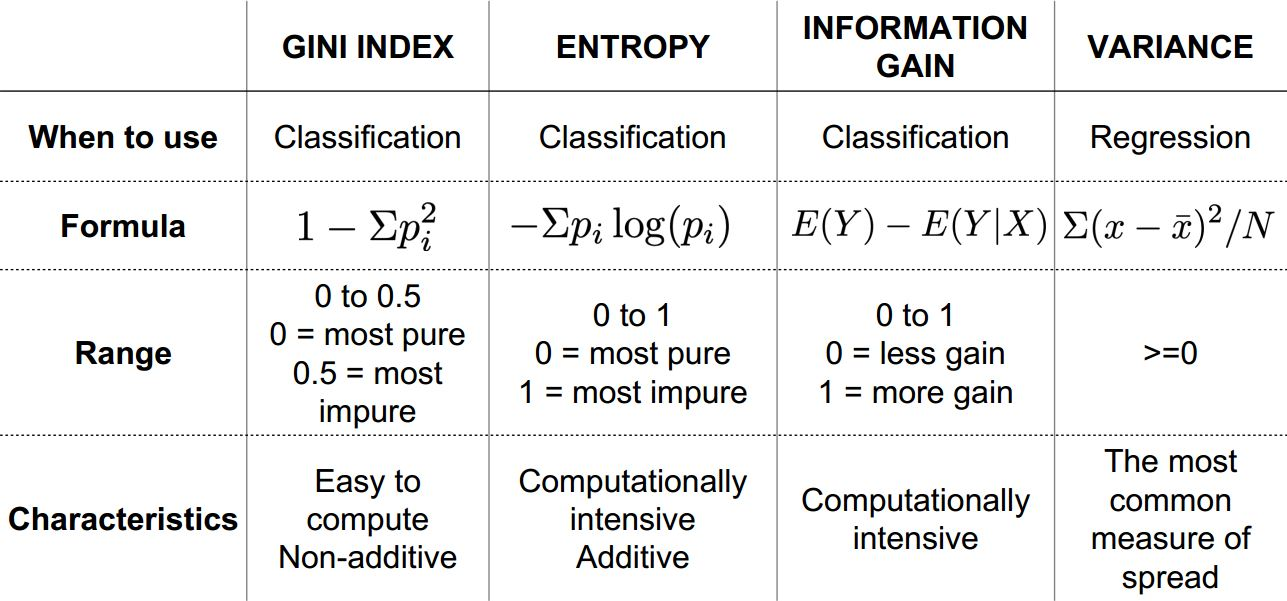
\includegraphics[width=\textwidth]{impuritymeasures}
		%\caption{}
		%\label{fig:}
	\end{figure}

There are several decision tree types, mostly they vary based on the measure of impurity used.  Some popular ones are:
	\begin{bulletedlist}
		\item CART: gini impurity
		\item C4.5: entropy
		\item CHAID: chi-squared
	\end{bulletedlist}

	\subsubsection{Gini Impurity}
Gini impurity how often is a randomly chosen element from the set would be incorrectly labeled if it was randomly labeled according to the distribution of labels in the subset.

Can be computed by summing the probability of an item with label $i$ being chosen ($p_i$), times the probability of a mistake ($1-p_i$)
in categorizing that item.
Simplifying gives, the Gini impurity of a set:
	\begin{equation}
		G(k) = 1 - \sum_{i=1}^J p_i^2
	\end{equation}

	\subsubsection{Entropy}
Entropy log is usually base 2, but it does not have to be.  Any log base can be chosen so long as it is consistent.

	\subsubsection{Information Gain}
	\begin{equation}
		E(Y) - E(Y|X)
	\end{equation}
	\begin{mathwhere}[0.4in]
		\mathdefitem{E(Y)}{entropy of the parent node;}
		\mathdefitem{E(Y|X)}{entropy of the combined children nodes.}
	\end{mathwhere}
Parent should have large entropy; the children should be purer and therefore have less entropy.

	\subsection{Cross Validation}
Cross Validation is a common Machine Learning technique that splits the data into n non-overlapping groups, and runs $n$ experiments:
	\begin{bulletedlist}
		\item In each experiment, $n-1$ groups are used to train a model and the model is tested on the left out group.
		\item The results are summarized over the $n$ experiments.
		\item It gives a mechanism that allows us to test a model repeatedly on data that was not used to build the model.
		\item For Decision Trees, a very common approach is simply to choose the tree with minimum cross validation error.
	\end{bulletedlist}

	\subsection{Pruning}
	\subsubsection{Pre-pruning}
Hyperparameters are specified before running the model.  Some hyperparameters in decision trees are:
	\begin{bulletedlist}
		\item max\_depth - The maximum depth of the tree. If set to ``None'', then nodes are expanded until all leaves are pure. Higher the value, more complex the tree.
		\item min\_samples\_split - The minimum number of samples required to split a node. Doesn't split any node that is smaller than this number. Higher the values, less complex the tree.
		\item min\_samples\_leaf - The minimum number of samples required at a leaf node. All leaf nodes have at least these many data points. Higher the value, less complex the tree.
	\end{bulletedlist}

Algorithms can search for the best hyperparameters to use (a grid search).  This can easily lead to over fitting the data.

	\subsubsection{Post-pruning}
Cost-complexity pruning.
	\begin{equation}
		\alpha = \frac{e_p - e_o}{n_r}
	\end{equation}
	\begin{mathwhere}[0.4in]
		\mathdefitem{e_p}{error on the pruned tree (always larger than $e_o$);}
		\mathdefitem{e_o}{error on the original tree;}
		\mathdefitem{n_r}{number of nodes reduce.}
	\end{mathwhere}
The smaller the $\alpha$ the smaller the value added by the subtree removed.  Remove the smallest $\alpha$ to create a new tree that has reduced nodes but is almost as accurate.

A small $\alpha$ means a complex model with lots of nodes.

	\begin{bulletedlist}
		\item Starting from the Full tree, create a sequence of trees that are sequentially smaller (pruned).
		\item At each step the algorithm
		\item try removing each possible subtree
		\item find the ``relative error decrease per node'' for that subtree Complexity parameter,
		\item And remove the subtree with the minimum
		\item With the list of subtrees, one usually reverts back to using cross validation errors to find the best final pruned tree.
	\end{bulletedlist}

	\begin{figure}[tbp]
		\begin{minipage}[t]{0.475\textwidth}
			\flushleft
			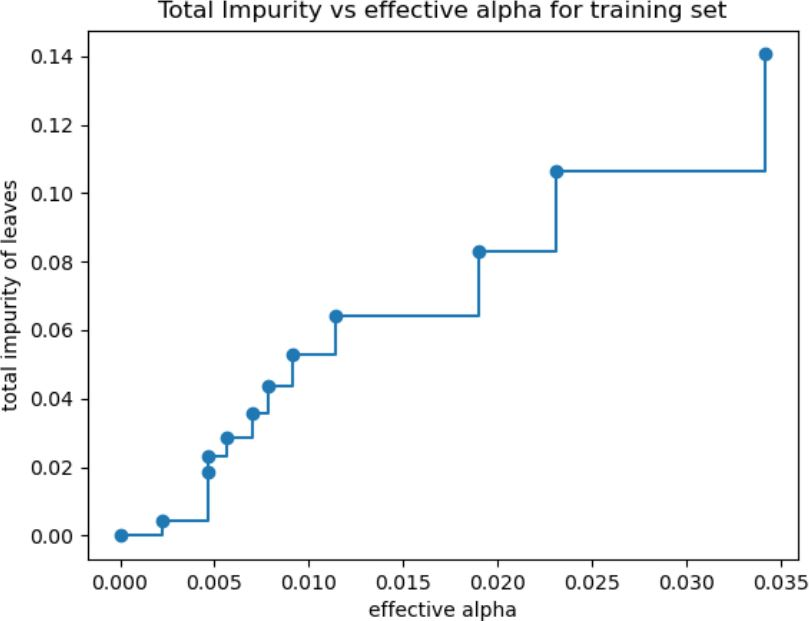
\includegraphics[width=\textwidth]{impurityversusalpha}
			%\caption{}
			%\label{fig:}
		\end{minipage}
		\hfill
		\begin{minipage}[t]{0.475\textwidth}
			\flushright
			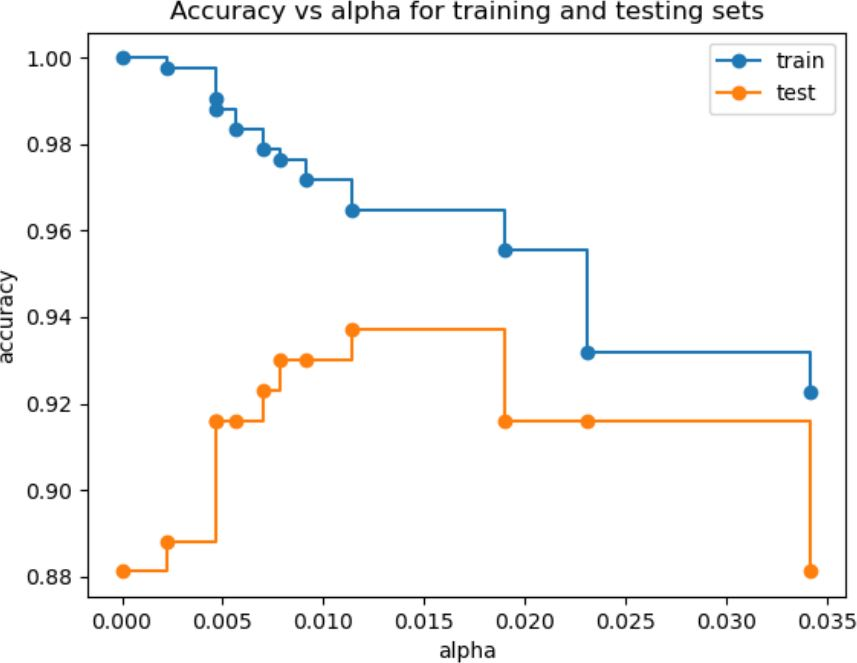
\includegraphics[width=\textwidth]{accuracyversusalpha}
			%\caption{}
			%\label{fig:}
		\end{minipage}
	\end{figure}


